\section{Meta-Learning}
%----------------------------------------------------------------------
%----------------------------------------------------------------------
\begin{frame}[c]{Meta-Learning: Introduction}

\begin{itemize}
	\item Learning essentially never stops:
	\begin{itemize}
		\item Many models are periodically re-fit to track changes in the data
		\item Many models are re-fit to perform well on new tasks
	\end{itemize}
	
    \item Learning is often done from scratch
    
    \item We humans do not start from scratch all the time \\ - we learned how to learn!
\end{itemize}

\end{frame}
%----------------------------------------------------------------------
%----------------------------------------------------------------------
\begin{frame}[c]{Meta-Learning: Introduction}

\begin{columns}
	\column{0.18\textwidth}
	Ren\'e Magritte
	\centering
	
\includegraphics[width=1.0\textwidth]{w07_hpo_grey_box/images/meta_learning/magritte_1.jpg}
	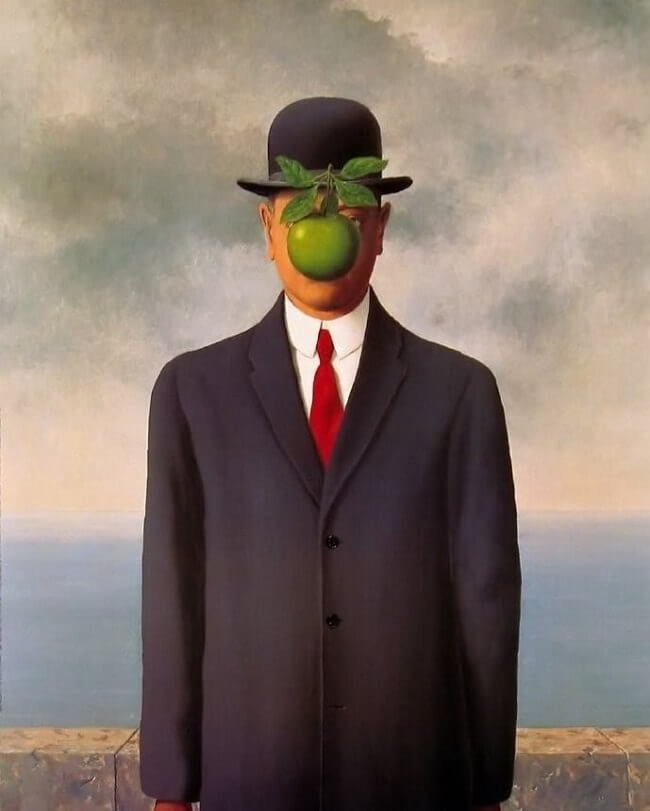
\includegraphics[width=1.0\textwidth]{w07_hpo_grey_box/images/meta_learning/magritte_2.jpg}
	\column{0.258\textwidth}
	Francis Picabia
	\centering
	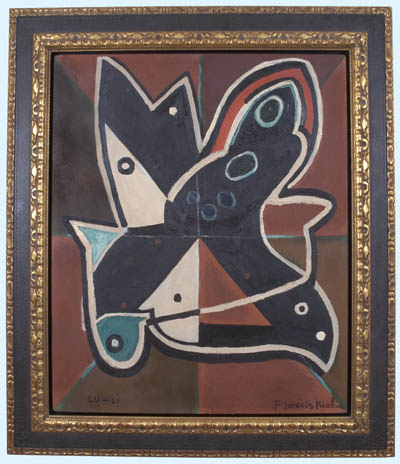
\includegraphics[width=.8\textwidth]{w07_hpo_grey_box/images/meta_learning/picabia_3.jpg}
	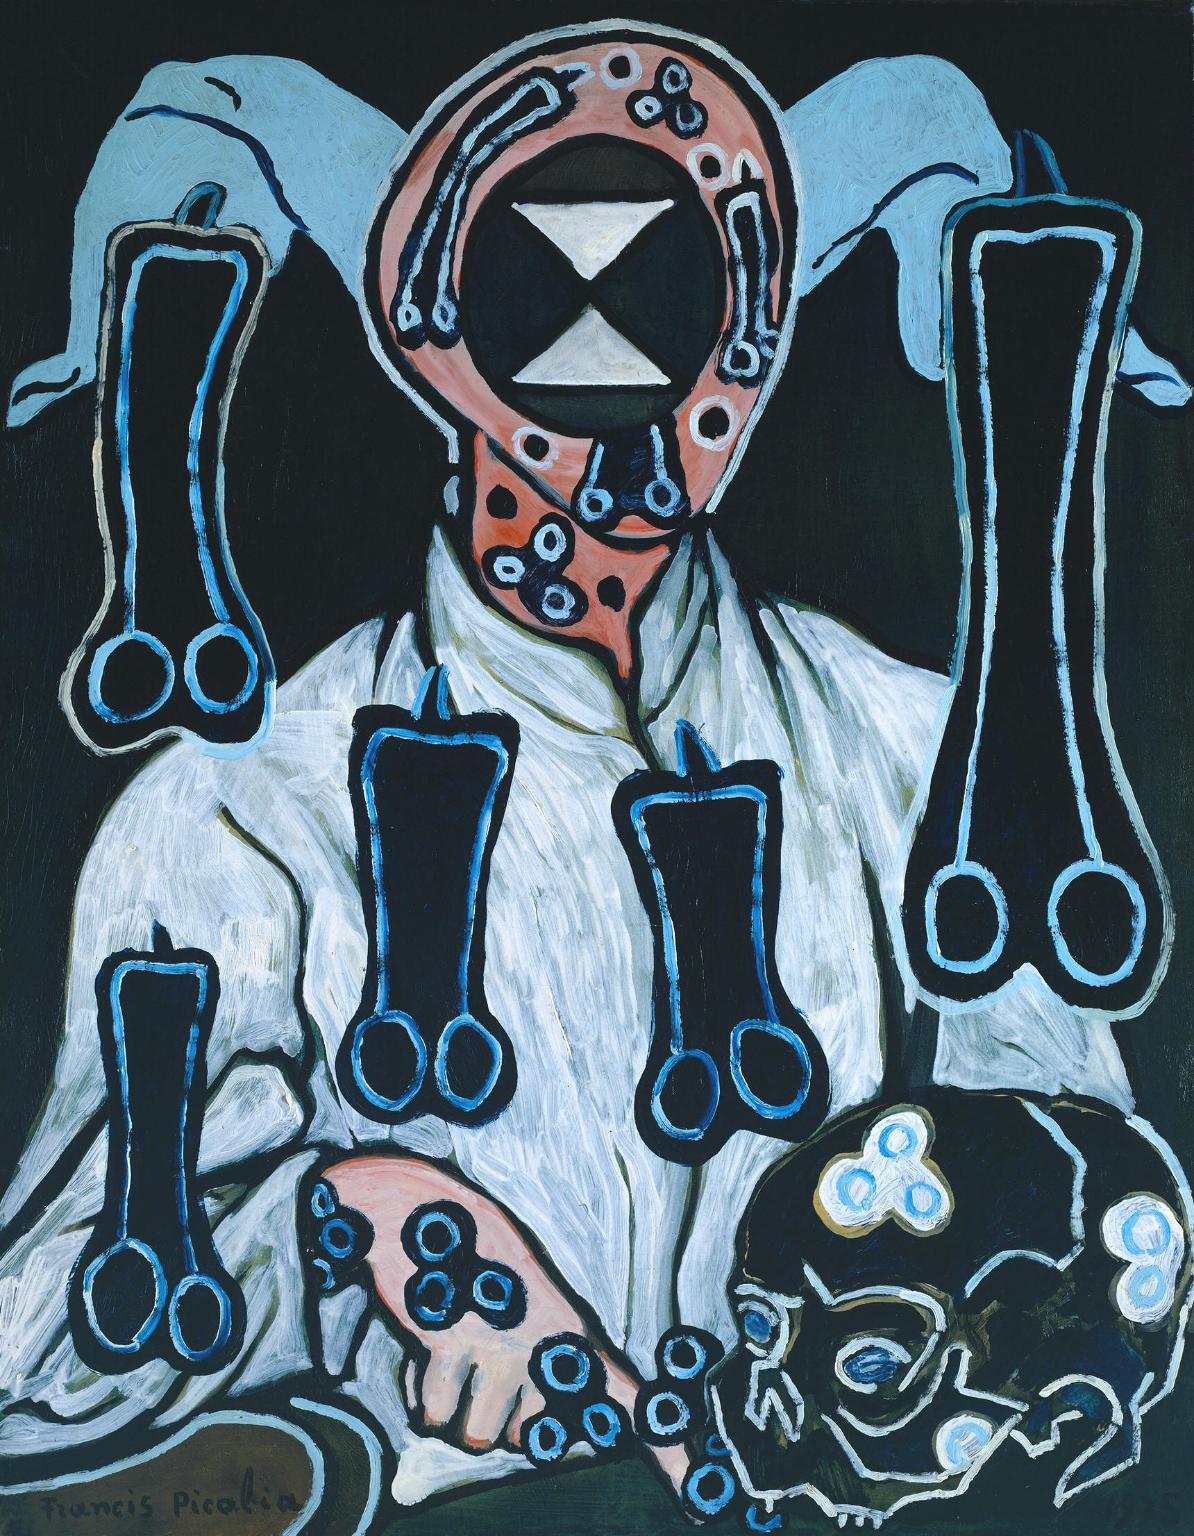
\includegraphics[width=.7\textwidth]{w07_hpo_grey_box/images/meta_learning/picabia_1.jpg}
	\column{0.3\textwidth}
	\centering
	Who painted that?
	
\includegraphics[width=.8\textwidth]{w07_hpo_grey_box/images/meta_learning/magritte_3.jpg}
	
	\pause
	Most likely most of you can identify the painter correctly, 
	although I presented only two pictures of each.
\end{columns}

\end{frame}
%----------------------------------------------------------------------
%----------------------------------------------------------------------
\begin{frame}[c]{Meta-Learning: Supervised Learning revisited}

Dataset:
\begin{equation*}
\dataset = \{(x_1, y_1), \ldots, (x_k, y_k) \}
\end{equation*}

\bigskip
\pause

Learning a model $\phi$ (e.g., weights of a neural network):
\begin{eqnarray*}
\argmax_{\phi} \log p(\phi|\dataset)\\
\pause
= \argmax_{\phi} \log p(\dataset | \phi) + \log p(\phi) \\
\pause
= \argmax_{\phi} \sum_i \log p(y_i | x_i, \phi) + \log p(\phi)
\end{eqnarray*}

\pause

Challenge:
\begin{itemize}
	\item Learning starts from scratch
	\item We might only have very few examples in $\dataset$ 
\end{itemize}

\end{frame}
%----------------------------------------------------------------------
%----------------------------------------------------------------------
\begin{frame}[c]{Meta-Learning: Problem formulation}

Dataset:
\begin{equation*}
\dataset = \{(x_1, y_1), \ldots, (x_k, y_k) \}
\end{equation*}
Set of datasets (meta-datasets):
\begin{equation*}
\mdata = \{\mathcal{D}_1, \ldots, \mathcal{D}_n, \}
\end{equation*}

\pause
Can we include these meta-datasets to improve learning on $\dataset$?
\begin{equation*}
\argmax_{\phi} \log p(\phi|\dataset, \mdata)
\end{equation*}

\pause
\medskip

\alert{Idea:} Instead of keeping $\mdata$ forever, we want to distill the knowledge into \alert{meta-parameters $\theta$}: $p(\theta|\mdata)$
 
\end{frame}
%----------------------------------------------------------------------
%----------------------------------------------------------------------
\begin{frame}[c]{Meta-Learning: Problem formulation}

In meta-learning, we want to learn:
\begin{eqnarray*}
\argmax_{\phi} \log p(\phi|\dataset, \mdata) \\
\pause
= \argmax_{\phi} \log \int_{\Theta} p(\phi \mid \dataset, \theta) p(\theta \mid \mdata) d\theta\\
\pause
\approx \argmax_{\phi} \log p(\phi | \dataset, \theta^*) + \log p(\theta^* | \mdata)\\
\pause
= \argmax_{\phi} \log p(\phi | \dataset, \theta^*)
\end{eqnarray*}

\pause

\begin{center}
\begin{minipage}{0.5\textwidth}
\begin{block}{Meta-learning problem}
\begin{equation*}
\theta^* \in \argmax_{\theta} \log p(\theta | \mdata)
\end{equation*}
\end{block}
\end{minipage}
\end{center}

\end{frame}
%-----------------------------------------------------------------------
%-----------------------------------------------------------------------
\begin{frame}[c]{Meta-Learning: AutoML $\subset$ Meta-Learning}

\begin{itemize}
	\item AutoML can be seen as a special case of meta-learning \pause
	\medskip
	\item $\theta$ could be:
	\begin{itemize}
		\item a hyperparameter configuration ($\lambda$) 
		\item a neural network architecture
	\end{itemize}
	\pause
	\medskip
	\item What would be $\mdata$ here? 
	\pause
	\begin{itemize}
		\item A dataset on which we optimized $\lambda$ (e.g. CIFAR-10)\\ such that we can use it on another dataset (e.g. imagenet)
	\end{itemize}
\end{itemize}	

\end{frame}
%-----------------------------------------------------------------------
%-----------------------------------------------------------------------
\begin{frame}[c]{Meta-Learning: Meta-Learning $\subset$ AutoML}

\begin{itemize}
	\item Meta-learning can be powerful to complement AutoML
	\pause
	\medskip
	\item We can learn a lot of things from $\mdata$ to improve the performance on new datasets, e.g.:
	\begin{itemize}
		\item pre-initialization of networks weights
		\item learning a meta-DNN to predict how to train another target-DNN	\end{itemize}
\end{itemize}	

\end{frame}
%-----------------------------------------------------------------------
%-----------------------------------------------------------------------
\begin{frame}[c]{Meta-Learning: Meta-Features in Machine Learning}
	
Based on their types and underlying assumptions, meta-features can be divided into at least five groups:
\pause
\begin{itemize}
	\item \alert{Simple meta-features} - number of features, patterns or classes, describe the basic dataset structure. \pause
	\item \alert{PCA meta-features} - compute various statistics of the datasets principal components. \pause
	\item \alert{The information-theoretic meta-features} - measure the class
entropy in the data. \pause
	\item \alert{Statistical meta-features} - characterize the data via descriptive statistics (e.g. the kurtosis or the dispersion of the label distribution).\pause
	\item \alert{Landmarking meta-features} - computed by running several
fast machine learning algorithms on the dataset. Based on
their learning scheme they can capture different properties
of the dataset, like e.g. linear separability.
\end{itemize}

\end{frame}
%-----------------------------------------------------------------------
%-----------------------------------------------------------------------
\begin{frame}[c]{Meta-Learning: Warmstarting}
	
\begin{itemize}
	\item Recap: Instead of starting from a random configuration we often start from a expert-defined configuration for hyperparameter optimization (HPO)
	\pause
	\item We also know that the default configuration often does not perform well on a new dataset
	\begin{itemize}
		\item Otherwise there would be no point in HPO
	\end{itemize}
	\pause
	\item \alert{Can we learn from previous datasets $\mdata$ how to initialize HPO?}\\
	(i.e., running an initial design)
	\begin{itemize}
		\item the same ideas also apply to NAS
		\item for simplicity we focus on HPO 
	\end{itemize}
\end{itemize}

\end{frame}
%-----------------------------------------------------------------------
%-----------------------------------------------------------------------
\begin{frame}[c]{Meta-Learning: Warmstarting}
	
\comment{Should we include some graphs for warmstarting?}

\end{frame}
%-----------------------------------------------------------------------
%-----------------------------------------------------------------------
\begin{frame}[c]{Meta-Learning: Learning Acquisition Functions}

\begin{itemize}
	\item Instead of learning everything, it might be sufficient to \alert{learn hand-design heuristics}
	\pause
	\item In Bayesian Optimization (BO), the most critical hand-design heuristic is the acquisition function
	\begin{itemize}
		\item trade-off between exploitation and exploration
		\item Depending on the problem at hand, you might need a different acquisition function
		\pause
		\item Choices:
		\begin{itemize}
			\item probability of improvement (PI)
			\item expected improvement (EI)
			\item upper confidence bounds (UCB)
			\item entropy search (ES) 
			\item knowledge gradient (KG)
			\item ...
		\end{itemize} 
	\end{itemize}
	\pause
	\item \alert{Idea:} Learn a \emph{neural acquisition function} from data
\end{itemize}

$\leadsto$ Replace acquisition function 

\source{Volpp et al.'19}

\end{frame}
%-----------------------------------------------------------------------
%-----------------------------------------------------------------------
\begin{frame}[c]{Meta-Learning: Learning Acquisition Functions}
	
Although the \alert{acquisition function $\alpha$} depends on the history $\mathcal{D}_{\bocount-1}$ and the predictive model $\surro$, $\alpha$ mainly makes use of the \alert{predictive mean $\mu$ and variance $\sigma^2$}.

\pause
\bigskip

Neural acquisition function (AF):

\begin{eqnarray}
\acq_\theta(x) = \acq_\theta(\mu_t(x), \sigma_t(x)) \nonumber
\end{eqnarray}

where $\theta$ are the parameters of a neural network,\\ and $\mu$ and $\sigma$ are its inputs.

\pause 
\begin{itemize}
	\item Since the input is not $x$, it allows to learn scalable acquisition function
	\item No calibration of hyperparameter necessary, once the neural AF is learnt
\end{itemize}

\end{frame}
%-----------------------------------------------------------------------
%-----------------------------------------------------------------------
\begin{frame}[c]{Meta-Learning: Learning Acquisition Functions}
	
\comment{Do you want to include this topic? (I did so we can easily delete it)}

\end{frame}
%-----------------------------------------------------------------------
%-----------------------------------------------------------------------

%-----------------------------------------------------------------------
%-----------------------------------------------------------------------
\begin{frame}[c]{Meta-Learning: Task-independent recommendations}



\begin{columns}[T] % align columns
\begin{column}{.48\textwidth}

    \begin{itemize}
        \item<1-7> \emph{Idea:} learn a sorted list of defaults
        \item<2-7> \emph{Method:} mostly greedy 
        \item<3-7> \emph{Results:} improves over Random Search and Bayesian Optimization
    \end{itemize}

    \only<4-7>{
    \begin{block}{Advantages}
    \begin{itemize}
    	\item<4-7> Easy to share and use
    	\item<5-7> Strong anytime performance
    	\item<6-7> Embarrassingly parallel
    \end{itemize}
    \end{block}}
    
    \only<7-7>{
    \begin{block}{Disadvantages}
    \begin{itemize}
    	\item<7-7> Not adaptive
    \end{itemize}
    \end{block}}

\end{column}%

\hfill%

\begin{column}{.48\textwidth}

    \centering
    \only<1-2>{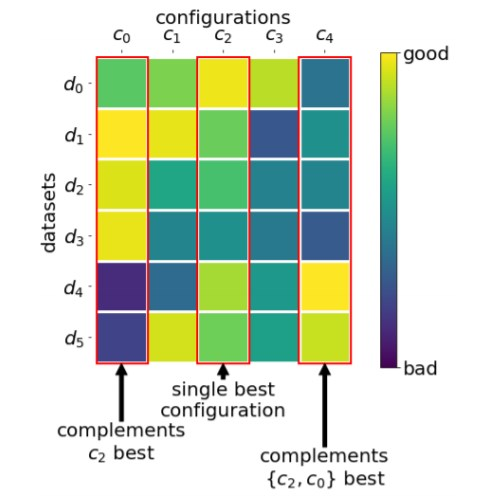
\includegraphics[width=.8\textwidth]{w07_hpo_grey_box/images/meta_learning/task_independent.jpg}}
    \only<3-7>{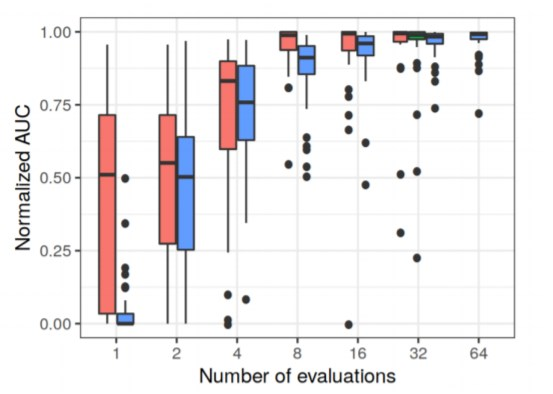
\includegraphics[width=.9\textwidth]{w07_hpo_grey_box/images/meta_learning/task_independent_results.jpg}}


\end{column}
\end{columns}  

\source{Wistuba et al., 2015a,\&b, Feurer et al., 2018, Pfisterer et al., 2018}

\end{frame}
%-----------------------------------------------------------------------
%-----------------------------------------------------------------------



%-----------------------------------------------------------------------
%-----------------------------------------------------------------------
\begin{frame}[c]{Meta-Learning: Joint model for Bayesian optimization}

\begin{columns}[T] % align columns
\begin{column}{.38\textwidth}

\begin{itemize}
    \item<1-5> Jointly train a „deep“ neural network on all tasks 
    \item<2-5> Have a separate output layer (head) for each tasks 
    \item<3-5> Each head is a Bayesian linear regression 
    \item<4-5> Feature extraction on hyperparameter configurations 
    \item<5-5> (Recall DNGO)
\end{itemize}
\end{column}%

\hfill%

\begin{column}{.58\textwidth}
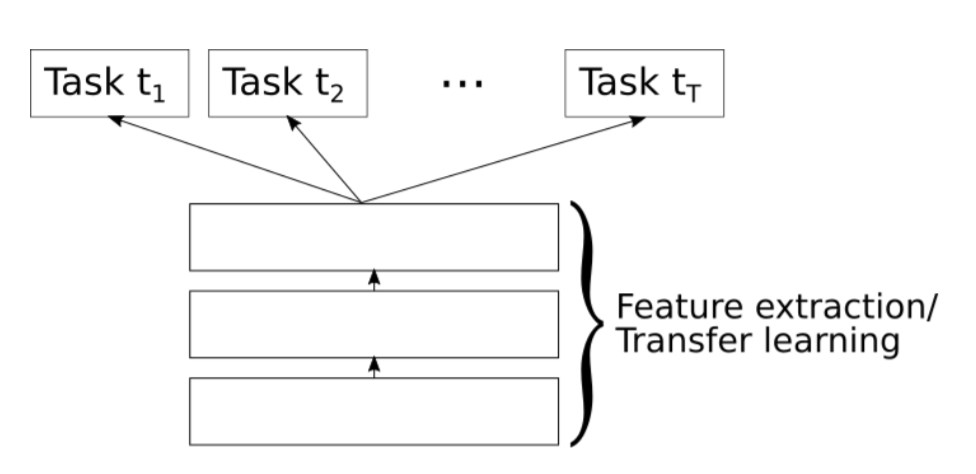
\includegraphics[width=0.9\textwidth]{w07_hpo_grey_box/images/meta_learning/perrone_int.jpg}
\end{column}%
\end{columns}

\source{Perrone et al. 2018}

\end{frame}
%-----------------------------------------------------------------------
%-----------------------------------------------------------------------
\begin{frame}[c]{Meta-Learning: Joint model for Bayesian optimization}
	
\centering
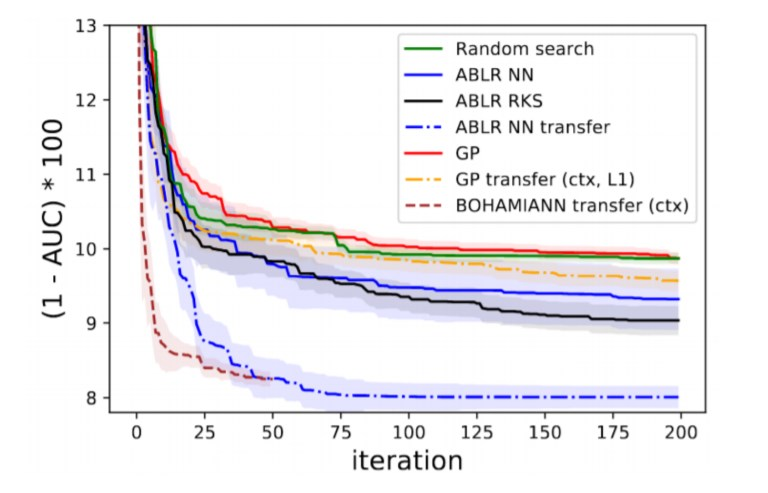
\includegraphics[width=0.7\textwidth]{w07_hpo_grey_box/images/meta_learning/perrone_res.jpg}

\end{frame}
%-----------------------------------------------------------------------
%-----------------------------------------------------------------------
